\section{Introduction}

$\Lambda$CDM cosmology is very successful at describing the Universe. However there remain many outstanding problems in the model that beg for a solution. One problem is the mysterious origin of the large-scale magnetic fields permeating the cosmos. Detections of Faraday rotation, synchrotron emissions and Zeeman splitting in distant galaxies and throughout intracluster media reveal weak magnetic fields, on the order of microgauss coherent over the scale of megaparsecs. Though there are models for describing the amplification of existing magnetic fields, such as magnetohydrodynamics and galactic dynamos there is no clear answer for where these magnetic fields came from.
\\\\
A possible answer to this question are primordial magnetic fields (PMFs). PMFs are seed magnetic fields produced in the early Universe sometime before recombination. These weak seed fields - of order nanoguass - could be taken up by galactic dynamos to become the weak magnetic field we see today. So far PMFs remain undetected, but with the next generation of CMB experiments and beyond beginning over the next decade, it is important to know how sensitive these experiments are to the faint traces of PMFs and whether they are able to make a detection.
The aim of this thesis is to forecast the upper-limits on PMF detections for stage-3 and stage-4-like CMB experiments.
\\\\
In this chapter I will begin by discussing the nature of the large-scale magnetic fields and the physics behind their amplification due to galactic dynamos in section 2.1. In section 2.2 I will discuss recent advances in constraining the PMF strength. Next, in section 2.3 I will give a quick review on CMB observables, polarisation and power spectra - which are instrumental in the study of PMFs. Finally in section 2.4 I will discuss CMB-S3 experiments with focus on the SPT-3G and Advanced ACTPol as well as preliminary figures on CMB-S4 experiments.

\subsection{Large Scale Magnetic Fields}

Galaxy clusters and their resident galaxies are known to possess weak microgauss magnetic fields coherent over scales as large as megaparsecs. Observational evidence of these magnetic fields come in the form of Zeeman splitting, synchrotron emission and Faraday rotation.
\subsubsection*{Zeeman Splitting}
\\
In the presence of magnetic fields, electronic energy levels in molecules and atoms split based on the angular momentum of the electron with respect to the orientation of the magnetic field. As a result, Zeeman splitting causes the spectral lines from distant sources to also split. Splitting of the Hydrogen 21cm line and the OH 18cm line are common probes of magnetic fields in our owng galaxy. Currently Zeeman splitting has given no constraints on the magnetic fields in the ICM. Zeeman splitting has been used to measure the magnetic fields within dense gas clouds around other galaxies, with strengths in the order of 0.5-18mG \cite{Robishaw:2008ti}, however these regions are not representative of the large-scale magnetic fields threading the cosmos.
\subsubsection*{Synchrotron Emissions}
\\
As electrons and ions spiral around magnetic fields in galaxies and the intracluster medium they emit synchrotron radiation with energies proportional to the strength of the magnetic field and the velocity of the ions.
\\
The emissivity of synchrotron radiation is given by:
\begin{equation}
j(B_{\bot},\nu) \propto n_0 B_{\bot}^{(1+\alpha)/2} \nu ^{(1-\alpha)/2}
\end{equation}
Where $\nu$ is the frequency of the electron's circular motion, $B_{\bot}$ is the magnetic field component perpendicular to the line of sight and $n_0$ is the normalised electron density, given by $n_e dE = n_0 E^{-\alpha} dE$ where E is the energy of the electron and $\alpha$ is the spectral index, the value for which varies from galaxy to galaxy.
\\
Synchrotron emissions from nearby galaxies have given constraints on $B_{\bot}$ within the range 4 $\mu G$ to 19 $\mu G$ \cite{Giovannini:2003yn}.
\subsubsection*{Faraday Rotation}
\\
As a polarised photon travels through a magnetised plasma it undergoes Faraday Rotation. Magnetised plasmas such as the intracluster medium exhibit different refractive indices for left and right circularly polarised light. Hence, as linearly polarised light propagates through the plasma, its plane of polarisation is rotated by some some angle, $\beta$, given by:

\begin{equation}
\beta = RM\lambda^2
\end{equation}
\\
where $\lambda$ is the wavelength of the photon and $RM$ is the rotation measure, given by:

\begin{equation}
RM = \frac{e^3}{2\pi ^2 \epsilon_0 m^2 c^3}\int_{0}^{d} n_e(s) B_{\|}(s) ds
\end{equation}
\\
The angle of rotation therefore depends on the electron density, $n_e$ in the plasma, the component of the magnetic field parallel to the direction of propagation of the photon, $B_{\|}$ and the photon's wavelength, $\lambda$.
\\\\
Measurements of Faraday rotation within galaxy clusters have found the magnetic field strength to lie in the range of 0.2 - 3 $\mu G$ \cite{Widrow:2002ud}. In additon, Faraday rotation measurements yield magnetic field strengths in galaxies as 4 - 6 $\mu G$ for spiral galaxies and 6 - 8 $\mu G$ in elliptical and irregular galaxies \cite{Widrow:2002ud}.

\subsubsection*{Galactic Dynamos}
\\
On their own, seed magnetic fields such as PMFs are too weak (of order nanoguass) to give rise to the magnetic fields we see in the cosmos today. There must be a process for amplifying the seed magnetic fields. \\Galactic dynamos are good candidates for seed magnetic field amplifiers. Dynamos are systems that convert kinetic energy into electromagnetic energy. Hot ionised gas rotates around the galactic centre of a galaxy. The ions drag the magnetic field lines along with them, tangling them up and increasing the magnetic flux density, and in addition the magnetic field strength. Hence galactic dynamos are able to amplify a weak seed magnetic field into a stronger magnetic field that we observe today.

\subsection{CMB Polarisation}
In the last decade CMB polarisation has proven a powerful tool for studying large scale strucutre and the early Universe. If PMFs did in fact exist, then their traces ought to be found within the CMB polarisation. Section 2 contains a discussion on how PMFs affect CMB polarisation.
\\\\
The CMB is the light from the Big Bang, however the CMB itself didn't form until 300,000 years after the Big Bang. At this point in time the Universe was cool enough to allow photons to decouple from baryons. This event is known as last-scattering. From there on the photons were able to free stream through the cosmos. Over the intervening 13 billion years the CMB photons have been cosmologically redshifted into the microwave frequency band. The CMB is a blackbody spectrum corresponding to a temperature of ~2.73K.

\\The polarisation of the CMB first arose due to quadrupolar temperature anisotropies at last scattering \cite{Hu:1997hv}. Thomson scattering of photons in the electron-photon plasma linearly polarises out-going photons, however without anisotropies or only dipolar anisotropies, the net polarisation of the CMB is cancelled out. An electron in the plasma is surrounded by two hot regions and two cool regions oriented perpendicular to one another. Photons approaching from the hotter region impart their polarisation more strongly than those from cooler regions, producing net polarisations over patches of the sky. Figure 1 shows a diagram of Thomson scattering in a region with quadrupolar anisotropy.

\begin{figure}[h]
\centering
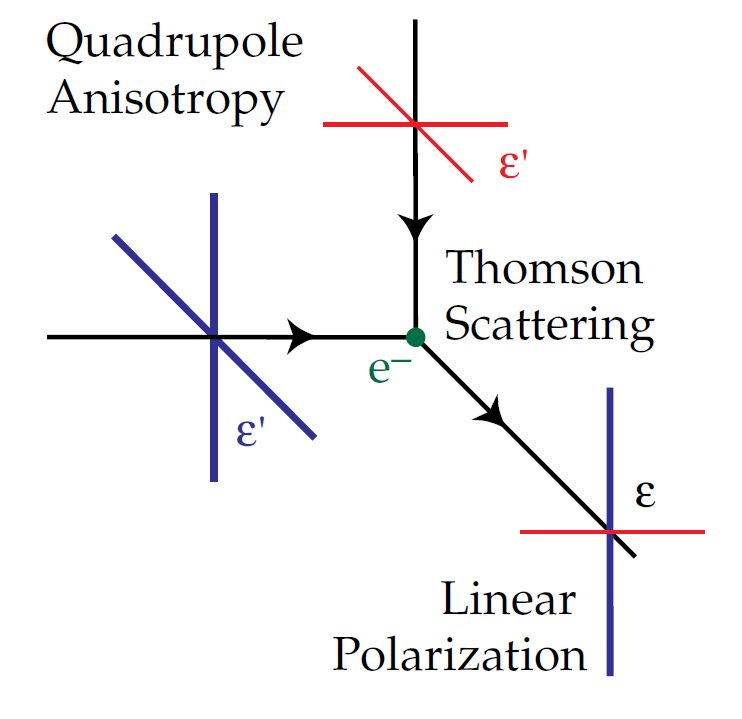
\includegraphics[scale=0.5]{thomson.png}
\caption{Thomson scattering of CMB photons in the presence of a quadrupole anisotropy. The red lines are the polarisations of a cold photon and the blue lines are the polarisations of a hot photon both incident on the same electron. The result is a net linear polarisation.}
\label{fig:thomson}
\end{figure}
\pagebreak
Quadrupolar anisotropies are caused by scalar, vector or tensor perturbations. Scalar perturbations are density fluctuations. Vector perturbations result from vortices in the photon-electron fluid or from more exotic phenomena, such as cosmic strings and other topologcal defects. Finally a tensor perturbation would be the result of gravity waves produced during cosmic inflation.  

In order to describe the effects of perturbations on CMB polarisation we introduce two polarisation modes. E-modes and B-modes. E-modes are formed from scalar perturbations. The E-modes resemble electric fields in electromagnetism in the sense that they are curl-free. It is also useful to note that E-modes have even parity. B-modes on the other hand are formed from vector and tensor perturbations and are currently undetected. Continuing the electromagnetism analogy a B-mode resembles a magnetic field, in the sense that it is purely a curl field. B-modes have odd parity.

\begin{SCfigure}
\centering
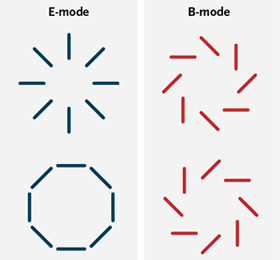
\includegraphics[scale=3]{modes.png}
\caption{Representation of E-mode polarisations and B-mode polarisations. Note how E-modes are symmetric and resemble a divergent field. In contrast the B-modes appear anti-symmetric and resemble a curled field.}
\label{fig:modes}
\end{SCfigure}

The causes of B-mode CMB polarisation are new frontiers in physics. There is a strong case to study CMB polarisation, in the hopes that we may shed some light on the exotic nature of the early Universe.

\subsubsection*{CMB Power Spectrum}

In studies of the CMB the power spectrum is a powerful tool. 

\\
The CMB angular power spectrum is defined as:
\begin{equation}
C_{\ell} = \frac{1}{2\ell + 1} \sum_{m = -\ell}^{\ell} \vert a_{\ell m} \vert ^2
\end{equation}
Where $a_{\ell m}$ is given by:
\begin{equation}
a_{\ell m} = \int_{4 \pi} T(\hat{n}) Y_{\ell m}^{*}(\hat{n})
\end{equation}


\subsection{Primordial Magnetic Fields}

As of yet PMFs remain undetected. 

The seed magnetic fields required to form the large-scale magnetic fields we see in the Universe today may have been primordial magnetic fields (PMFs). At some point in the evolution of the Universe a weak magnetic field with a strength less than a few nanogauss may have been produced. Recent work from PLANCK (2015) has constrained the primordial magnetic field strength coherent over 1 Mpc to $B_{1Mpc}$ $<$ 4.4nG \cite{Ade:2015cva}. In 2016 POLARBEAR modestly improved this constraint to $B_{1Mpc}$ $<$ 3.9nG \cite{Ade:2015cao}.

\iffalse
	- seed magnetic field produced in the early universe
	- undetected
	- predicted magnitude of < 1 nG.
	- evolves through magnetohydrodynamical processes
\fi


\subsection{Future CMB experiments}
This year stage-3 CMB experiments will commence operation and before the end of the next decade, stage-4 CMB experiments will have also collected their data. The next generation of CMB experiments aim to obtain tighter constraints on cosmological parameters such as the tensor-to-scalar ratio as well as map the CMB in higher detail than ever before. 

	- stage 3 of CMB experiments operating from 2016 to 2020.
	- n detectors, m detector years
	- primary science goal is to detect PGW from cosmic inflation through B-modes.
	- could also make a detection of PMFs.
\subsubsection{CMB-S3}
	
	
	- South Pole Telescope
	- n detectors
	- starting/finishing dates
	- area
	- etc.

\subsubsection{CMB-S4}
	- stage 4 CMB experiments still in planning stages - nothing concrete yet.
	- n detectors, m detector years
	- running through the 2020s